\documentclass[paper=a4,fontsize=9.0pt]{temp} % KOMA-article class	
\usepackage{amsfonts}
\usepackage{amssymb}
\usepackage{helvet}
\usepackage{hyperref}
\usepackage{url} %uso de url
\usepackage{xcolor}
\usepackage{multicol}%multicolumnas
\setlength{\columnsep}{0.1cm}
\usepackage{ marvosym }%iconos
\usepackage{fontawesome}%iconos 
\usepackage{amsmath} 
\setlength\parindent{0pt} %alineación a la izquierda
\usepackage{hyperref} % incluye url bajo una palabra cualquiera
\hypersetup
{
	%pdftoolbar=false, % toolbar hidden
	pdfmenubar=true, %menubar shown
	pdfhighlight=/O, %effect of clicking on a link
	colorlinks=true, %couleurs sur les liens hypertextes
	pdfpagemode=UseNone, %aucun mode de page
	pdfpagelayout=SinglePage, %ouverture en simple page
	linkcolor=linkcol, %couleur des liens hypertextes internes
	citecolor=citecol, %couleur des liens pour les citations
	urlcolor=URLcol %couleur des liens pour les url
}
% con este parametro se modifica el tamaño de la hoja segun queramos 
\usepackage{geometry}
 \geometry{
 a4paper,
 total={175mm,257mm},
 left=10mm,
 top=7mm,
 }
%%%%%%%%%%%%%%%%%%%%%%%%%%%%%%%%%%%%% inicio del documento %%%%%%%%%%%%%%%%%%%%%%%%%%%%%%%%%
\begin{document}
% %%%%%%%%%%%%%%%%%%%%%%%%%%%%%% inicio de los datos de contacto. %%%%%%%%%%%%%%%%%%
\begin{minipage}{0.28\linewidth}
   \MyName{ Miguel Salazar Reyes}
  
\vspace{1.0mm}

   {\faMapMarker \ \  Ciudad de Bogotá, Colombia} 

   {\faMobile \ \  {(+57) 318 889 25 10}}
   
   {\faEnvelope \ \  \href{mailto:miguelsloan18@gmail.com}{miguelsloan18@gmail.com}}
      
    %{\Telefon \ \  {(+57) 601-452-34-87}}
   
   {\faLinkedinSquare \ \  \href{https://www.linkedin.com/in/miguel-salazar-reyes/}{miguel-salazar-reyes}}
   
{\faGithub  \ \  \href{https://github.com/miguelsalazar18}{miguelsalazar18}}

\end{minipage}
%%%%%%%%%%%%%%%%%%%%%%  espacio para la foto por si acaso, se configura el espacio horizontal a la derecha, tamaño del espacio y de la foto %%%%%%%%%%%%%%%%%%%%%%%%%%%%%%%
\hspace{25.0mm}
\begin{minipage}{0.49\linewidth}
 \hfill{
\includegraphics[width=0.3\textwidth]{blanco1.PNG}}
\end{minipage}

% inicio primera columna de info 
\noindent
\begin{minipage}[c]{0.6\linewidth}
\NewPart{Perfil Profesional}{} % momento donde se examina si el perfil corresponde a lo que busca elempleador%%%%%%%%%%%%%%%%%%%%%%%
\noindent
Economista de la Universidad Nacional de Colombia. Con experiencia en investigación, análisis y extracción de información en grandes bases de datos, métodos de evaluación de impacto y seguimiento de mercados financieros; Office Avanzado y dominio del idioma inglés.
%%%%%%%%%%%%%%%%%%%%%%%%%%%%%%%%%%%%%%%%%%%%%%%%%%%%%%%%%%%%%%%%%%%%%%%%%%%%%%%%
\NewPart{Experiencia Laboral}{}
\noindent

\workEntry{Autoridad Nacional de Licencias Ambientales}{\hspace{10.0mm}Jul -  2021}{\hspace{23.0mm}Economista}{\textbf{Funciones:} Elaboración de estudios económicos con impacto ambiental; construcción y seguimiento de indicadores de impacto ambiental.\hspace{70.0mm} \textbf{-} Implementación de metodologías e instrumentos para la planeación estratégica de los planes, programas y proyectos de la ANLA.
\\
\textbf{Logros}: 
Aportar en la creación de un programa nacional de reducciones de gases de efecto invernadero en entidades públicas. \hspace{70.0mm} \textbf{-} Participar en la creación de un concepto socioeconómico sobre la explotación de yacimientos no convencionales en el país. 

\\ \hspace{1.0mm}{}} {ANLA}

\workEntry{Congreso de la república}{\hspace{90.0mm}Ago - Abr 2021}{\hspace{23.0mm}Asesor económico}{\textbf{Funciones:} Realizar estudios económicos usados para la formulación de proyectos de ley.   
\\
\textbf{Logros}: 
Aportar en el fundamento económico para la formulación de proyectos de ley. Además de estructurar bases para iniciativas legislativas orientadas al diseño y cambio de políticas públicas.\hspace{70.0mm} \textbf{-} Contribuir en la estructuración de iniciativas legislativas presentadas por este despacho, identificando su impacto económico y social.

\\ \hspace{1.0mm}{}} {congres}

\workEntry{Econometría consultores}{\hspace{5.0mm} Abr - Jun 2020}{\hspace{11.0mm} Asistente de investigación}{\textbf{Funciones:} Búsqueda, análisis y redacción de documentos sobre la regulación normativa de los mercados energéticos internacionales.  
\\
\textbf{Logros:} 
Contribuir en la construcción de un concepto regulatorio aplicable al mercado energético colombiano en colaboración con la CREG.  

\\ \hspace{1.0mm}{}} {Econometria}

\workEntry{Ministerio de Hacienda y Crédito Público}{Jul - Dic 2019}{\hspace{30.0mm}Pasantía Universitaria}{\textbf{Funciones:} Monitoreo del mercado de renta fija, construcción de indicadores de renta fija, redacción de informes periódicos. 
\\
\textbf{Logros}: 
Diseñar herramientas en macros para facilitar la redacción de los informes de subastas de deuda interna de corto y largo plazo.
\\ \hspace{1.0mm}{}} {Logo_Minhacienda}


%\sepspace

\workEntry{Banco de la República de Colombia}{Ene - Jun 2019}{\hspace{30.0mm}Prácticas profesionales}{\textbf{Funciones:} Búsqueda y creación de bases de datos, creación de modelos económicos con software estadístico.
\\
\textbf{Logros}: Contribuir en la construcción y actualización de los datos usados en el documento publicado en \href{https://repositorio.banrep.gov.co/handle/20.500.12134/9698}{\textbf{Borradores de Economía; No. 1078}}   del Banco de la República

\\ \\\hspace{1.0mm}{}}{banrep}
%%%%%%%%%%%%%%%%%%%%%%%%%%%%%%%%%%%%%%%%%%%%%%%%%%%%%%%%%%%%%%%%%%%%%%%%%%%%%%%%
%\NewPart{Experiencia Académica}{}
%\noindent

%\EducationEntry{Monitor Académico }{Jul 2015 - Nov 2019}{Universidad Nacional de Colombia}{\textbf{Economía colombiana \\ Desarrollo Económico  \\Metodología de la investigación II}
\\
%Apoyar y complementar las clases magistrales.} {images}
%%%%%%%%%%%%%%%%%%%%%%%%%%%%%%%%%%%%%%%%%%%%%%%%%%%%%%%%%%%%%%%%%%%%%%%%%%%%%%%%%%
\NewPart{Educación}{}
\noindent

\EducationEntry{\hspace{4.2mm}Maestría en economía (PEG)}{\textit{En curso}}{\hspace{4.2mm}Universidad  de los Andes }{Enfoque en métodos de Big data, Machine Learning y economía aplicada.} {Los_Andes}

\sepspace

\EducationEntry{\hspace{4.2mm}Pregrado en economía}{May 2020}{\hspace{4.2mm}Universidad Nacional de Colombia}{Interés en temas econométricos, investigación económica y mercados financieros. Becario académico durante 3 años.} {2}

%\EducationEntry{Intercambio Académico}{jul 2018}{\hspace{3.0mm}Pontificia Universidad Javeriana }{Profundización en las áreas de macroeconomía y teorías del comercio Internacional.} {logo_javer_azul_sm}

%%%%%%%%%%%%%%%%%%%%%%%%%%%%%%%%%%%%%%%%%%%%%%%%%%%%%%%%%%%%%%%%%%%%%%%%%%%%%%%%%%%%%%%
\end{minipage} % no space if you would like to put them side by side
\hspace{6mm}
\noindent
\begin{minipage}[c]{0.38\linewidth}
%%%%%%%%%%%%%%%%%%%%%%%%%%%%%%%%%%%%%%%%%%%%%%%%%%%%%%%%%%%%%%%%%%%%%%%%%%%%%%%%%%%%%%%%5
\NewPart{Investigaciones}{}
\noindent

\sepspace

\sepspace

\EducationEntry{Impacto de la pandemia sobre el mercado laboral en Colombia}{\hspace{39mm}Nov - 2020}
{\href{https://drive.google.com/file/d/1_un0wtoSjGnYKQLilnq4tqaXhcPW0k6Z/view?usp=sharing}{\textbf{Documento escuela de economía 111 FCE}} }{}{}

\EducationEntry{Impacto de la pandemia covid-19 sobre
la economía colombiana.}{\hspace{39mm}Ago - 2020}{\href{https://drive.google.com/file/d/1rQZkDZED0Ym_ConeDeuYuw4x7tTJTpnq/view}{\textbf{Documento escuela de economía 108 FCE}}}{}{}

\sepspace

\sepspace

%%%%%%%%%%%%%%%%%%%%%%%%%%%%%%%%%%%%%%%%%%%%%%%%%%%%%%%%%%%%%%%%%%%%%%%%%%%%%
%\NewPart{Intereses}{}
%\noindent

%Econometría, tratamiento de datos, mercados financieros, análisis de políticas %públicas e investigación
%%%%%%%%%%%%%%%%%%%%%%%%%%%%%%%%%%%%%%%%%%%%%%%%%%%%%%%%%%%%%%%%%%%%%%%%%%%%%%%%
%\NewPart{Actividades}{}
%\noindent

%\sepspace

%\EducationEntry{Voluntariado FCE}{\hspace{14mm}Jun - Jul  2017}{\hspace{8.0mm}Universidad Nacional}{Apoyo a los nuevos admitidos a la facultad de ciencias económicas de la Universidad Nacional}{}
%%%%%%%%%%%%%%%%%%%%%%%%%%%%%%%%%%%%%%%%%%%%%%%%%%%%%%%%%%%%%%%%%%%%%%%%%%%%%
\NewPart{Fortalezas}{}
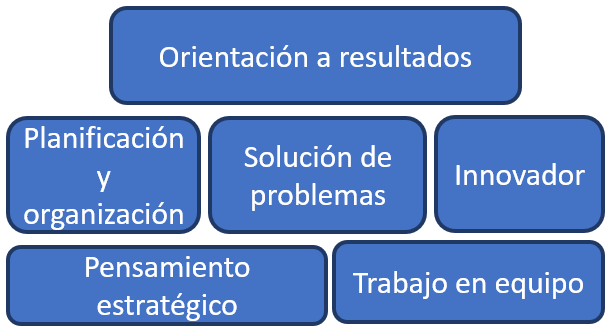
\includegraphics[width=1.02\textwidth]{fortalezas.png}
%%%%%%%%%%%%%%%%%%%%%%%%%%%%%%%%%%%%%%%%%%%%%%%%%%%%%%%%%%%%%%%%%%%%%%%%%
\NewPart{cursos}{}
\noindent
\EducationEntry{Data science & machine learning en python}{\hspace{39mm}May - Jun  2020}{Universidad Nacional}{Uso y análisis de información mediante el uso de algoritmos capaces de aprender}{}

% agregar $ $ para subir la columna 
%%%%%%%%%%%%%%%%%%%%%%%%%%%%%%%%%%%%%%%%%%%%%%%%%%%%%%%%%%%%%%%%%%%%%%%%%
\NewPart{habilidades}{}
\begin{minipage}[t]{0.1\textwidth} 				
\begin{tabular}[t]{l l}	
% %%%%%%%%%%%%%%%%%%%%%%%%% EXCEL %%%%%%%%%%%%%%%%%%%%%%%%%%%%%%
\hspace{5.0mm} \software{exce}  	 & Excel \hspace{18.0mm} \Huge{$\bullet$$\bullet$$\bullet$$\bullet$$\bullet$} \\
%%%%%%%%%%%%%%%%%%%%%%%%5 BLOOMBERG %%%%%%%%%%%%%%%%%%%%%%%%%%%%%%%%%%%
\hspace{5.0mm} \software{blom}  	 &Bloomberg \hspace{9.7mm} \Huge{$\bullet$$\bullet$$\bullet$$\bullet$\textcolor{lightgray}{$\bullet$}} \\	
%%%%%%%%%%%%%%%%%%%%%%%%%%% STATA %%%%%%%%%%%%%%%%%%%%%%%%%%%%%%%%%%%%
\hspace{5.0mm} \software{stata}  	 & Stata \hspace{18.0mm} \Huge{$\bullet$$\bullet$$\bullet$$\bullet$\textcolor{lightgray}{$\bullet$}}\\	
%%%%%%%%%%%%%%%%%%%%%%%%% R %%%%%%%%%%%%%%%%%%%%%%%%%%%%%%%%%%%%
\hspace{5.0mm} \software{r} 		 & R \hspace{23.4mm} \Huge{$\bullet$$\bullet$$\bullet$\textcolor{lightgray}{$\bullet$}\textcolor{lightgray}{$\bullet$}} \\
%%%%%%%%%%%%%%%%%%%%%%%% PYTHON %%%%%%%%%%%%%%%%%%%%%%%%%%%%%%
\hspace{5.0mm} \software{py} 		 & Python \hspace{15.4mm} \Huge{$\bullet$$\bullet$$\bullet$\textcolor{lightgray}{$\bullet$}\textcolor{lightgray}{$\bullet$}}\\
%%%%%%%%%%%%%%%%%%%%%%% MATHLAB %%%%%%%%%%%%%%%%%%%%%%%%%%%%%%
\hspace{5.0mm} \software{IMG/soft/Matlab}  	 & Matlab \hspace{15.5mm} \Huge{$\bullet$\textcolor{lightgray}{$\bullet$}\textcolor{lightgray}{$\bullet$}\textcolor{lightgray}{$\bullet$}\textcolor{lightgray}{$\bullet$}} \\	
	
\end{tabular}		
\end{minipage}
%%%%%%%%%%%%%%%%%%%%%%%%%%%%%%%%%%%%%%%%%%%%%%%%%%%%%%%%%%%%%%%%%%%%%%%%%%%%%%%%%%%%%%%%%%%%%%%%
\NewPart{lenguajes}{}
\hspace{3mm}
\begin{minipage}[t]{0.33\textwidth} 		
		
\begin{tabular}[t]{ l l }		
%%%%%%%%%%%%%%%%%%%%%%%%%%%%%%% ESPAÑOL %%%%%%%%%%%%%%%%%%%%%%%%%%%%%%
\hspace{9.5mm} \flag{IMG/flag/es}  & \hspace{4.5mm} \Huge{$\bullet$$\bullet$$\bullet$$\bullet$$\bullet$} \\		
%%%%%%%%%%%%%%%%%%%%%%%%%%%%%%%  INGLES %%%%%%%%%%%%%%%%%%%%%%%%%%%%%%
\hspace{9.5mm} \flag{IMG/flag/gb}  & \hspace{4.5mm} \Huge{$\bullet$$\bullet$$\bullet$\textcolor{lightgray}{$\bullet$}\textcolor{lightgray}{$\bullet$}}\\		
%%%%%%%%%%%%%%%%%%%%%%%%%%%%%%% ALEMAN %%%%%%%%%%%%%%%%%%%%%%%%%%%%%%
\hspace{9.5mm} \flag{IMG/flag/de}  & \hspace{4.5mm} \Huge{$\bullet$\textcolor{lightgray}{$\bullet$}\textcolor{lightgray}{$\bullet$}\textcolor{lightgray}{$\bullet$}\textcolor{lightgray}{$\bullet$}}\\	

\end{tabular}					
\end{minipage}	
%%%%%%%%%%%%%%%%%%%%%%%%%%%%%%%%%%%%%%%%%%%%%%%%%%%%%%%%%%%%%%%%%%%%%%%


\sepspace

\sepspace

\sepspace

\sepspace

\sepspace



\end{minipage}

\end{document}
